\section{eo\-Eval\-Func\-Ptr$<$ EOT, Fit\-T, Function\-Arg $>$ Struct Template Reference}
\label{structeo_eval_func_ptr}\index{eoEvalFuncPtr@{eoEvalFuncPtr}}
EOEval\-Func\-Ptr: This class takes an existing function pointer and converts it into a evaluation function class.  


{\tt \#include $<$eo\-Eval\-Func\-Ptr.h$>$}

Inheritance diagram for eo\-Eval\-Func\-Ptr$<$ EOT, Fit\-T, Function\-Arg $>$::\begin{figure}[H]
\begin{center}
\leavevmode
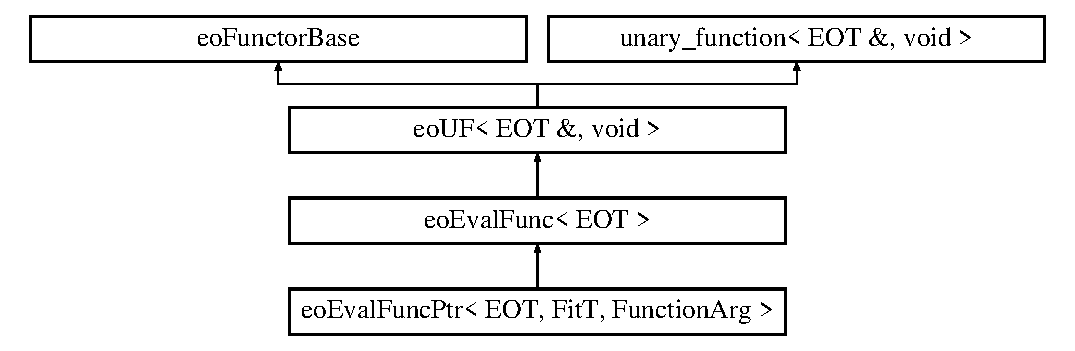
\includegraphics[height=4cm]{structeo_eval_func_ptr}
\end{center}
\end{figure}
\subsection*{Public Member Functions}
\begin{CompactItemize}
\item 
{\bf eo\-Eval\-Func\-Ptr} ({\bf Fit\-T}($\ast$\_\-eval)(Function\-Arg))
\begin{CompactList}\small\item\em Applies the function to the chromosome and sets the fitness of the Chrom. \item\end{CompactList}\item 
virtual void {\bf operator()} ({\bf EOT} \&\_\-eo)\label{structeo_eval_func_ptr_a1}

\begin{CompactList}\small\item\em Effectively applies the evaluation function to an {\bf EO}{\rm (p.\,\pageref{class_e_o})}. \item\end{CompactList}\end{CompactItemize}
\subsection*{Private Attributes}
\begin{CompactItemize}
\item 
{\bf Fit\-T}($\ast$ {\bf eval\-Func} )(Function\-Arg)\label{structeo_eval_func_ptr_r0}

\end{CompactItemize}


\subsection{Detailed Description}
\subsubsection*{template$<$class EOT, class Fit\-T = typename EOT::Fitness, class Function\-Arg = const EOT\&$>$ struct eo\-Eval\-Func\-Ptr$<$ EOT, Fit\-T, Function\-Arg $>$}

EOEval\-Func\-Ptr: This class takes an existing function pointer and converts it into a evaluation function class. 

That way, old style C or C++ functions can be adapted to {\bf EO}{\rm (p.\,\pageref{class_e_o})} function classes. 



Definition at line 43 of file eo\-Eval\-Func\-Ptr.h.

\subsection{Constructor \& Destructor Documentation}
\index{eoEvalFuncPtr@{eo\-Eval\-Func\-Ptr}!eoEvalFuncPtr@{eoEvalFuncPtr}}
\index{eoEvalFuncPtr@{eoEvalFuncPtr}!eoEvalFuncPtr@{eo\-Eval\-Func\-Ptr}}
\subsubsection{\setlength{\rightskip}{0pt plus 5cm}template$<$class EOT, class Fit\-T = typename EOT::Fitness, class Function\-Arg = const EOT\&$>$ {\bf eo\-Eval\-Func\-Ptr}$<$ {\bf EOT}, {\bf Fit\-T}, Function\-Arg $>$::{\bf eo\-Eval\-Func\-Ptr} ({\bf Fit\-T}($\ast$)(Function\-Arg) {\em \_\-eval})\hspace{0.3cm}{\tt  [inline]}}\label{structeo_eval_func_ptr_a0}


Applies the function to the chromosome and sets the fitness of the Chrom. 

Thus, the evaluation function need not be worried about that. \begin{Desc}
\item[Parameters:]
\begin{description}
\item[{\em \_\-eval}]pointer to the evaluation function, takes a EOT as an argument and returns the fitness \end{description}
\end{Desc}
\begin{Desc}
\item[Returns:]the evaluated fitness for that object. \end{Desc}


Definition at line 51 of file eo\-Eval\-Func\-Ptr.h.

The documentation for this struct was generated from the following file:\begin{CompactItemize}
\item 
eo\-Eval\-Func\-Ptr.h\end{CompactItemize}
